% Fig 1: Controller D overview. Black/gray plus one accent. Compile: tectonic fig1_overview.tex
\documentclass[tikz,border=2pt]{standalone}
\usepackage[T1]{fontenc}
\usepackage{helvet}
\renewcommand{\familydefault}{\sfdefault}
\usetikzlibrary{arrows.meta,positioning,calc}
\definecolor{acc}{HTML}{2a78d6}
\definecolor{g1}{gray}{0.2}
\definecolor{g2}{gray}{0.55}
\definecolor{g3}{gray}{0.86}
\tikzset{
  every node/.style={font=\fontsize{7.5}{9}\selectfont},
  box/.style={draw=g1, rounded corners=1.5pt, thin, fill=white, align=center, inner sep=2.5pt,
              minimum height=1.15cm, minimum width=2.0cm, text width=1.92cm},
  accbox/.style={box, draw=acc, fill=acc!10, very thick},
  arr/.style={-{Stealth[length=4pt]}, thin, draw=g1},
  accarr/.style={-{Stealth[length=4pt]}, thick, draw=acc},
  lab/.style={font=\fontsize{7}{8.2}\selectfont, text=g1},
  panel/.style={font=\fontsize{8.5}{10}\selectfont\bfseries, anchor=west},
}
\hyphenpenalty=10000 \exhyphenpenalty=10000
\begin{document}
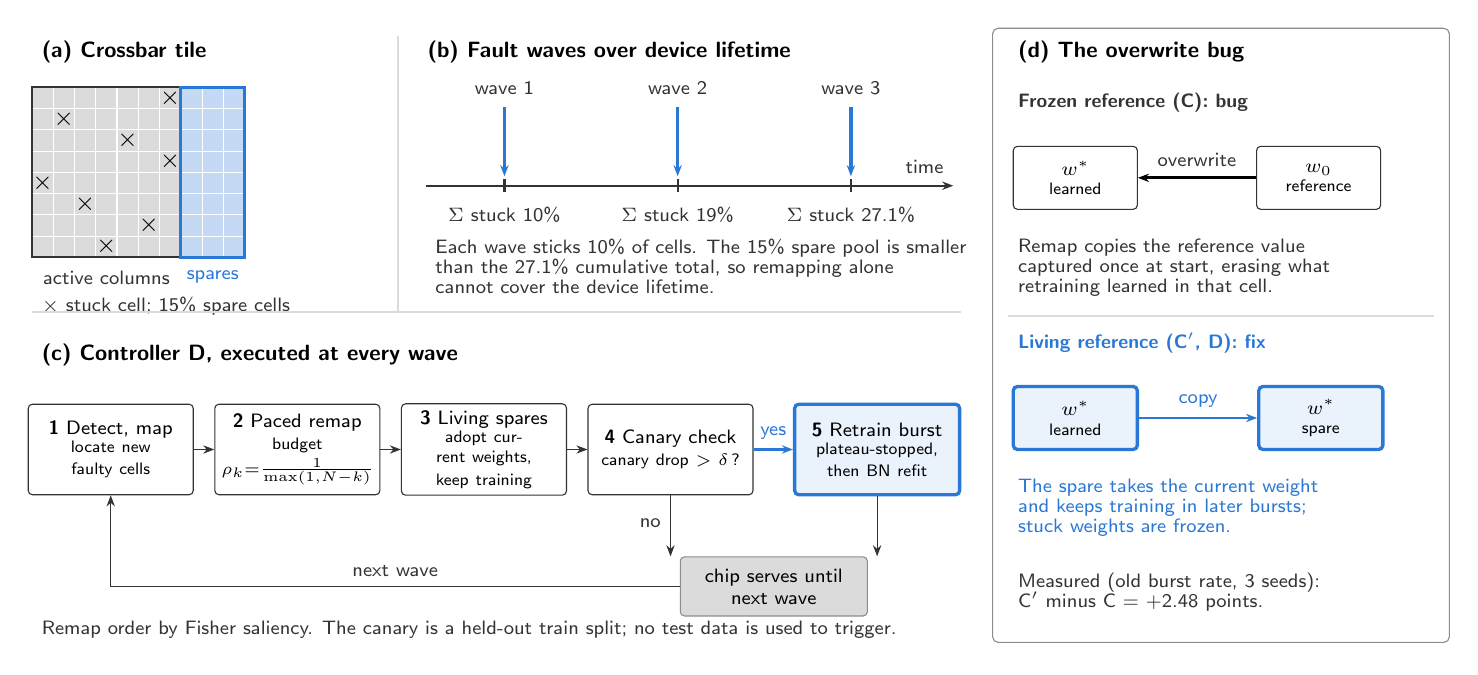
\begin{tikzpicture}[x=1cm,y=1cm]

%% ---------- (a) crossbar tile with spare columns ----------
\node[panel] at (0,7.8) {(a) Crossbar tile};
\def\cs{0.27}
\def\top{7.35}
\foreach \i in {0,...,6}{\foreach \j in {0,...,7}{
  \fill[g3,draw=white,thin] (\i*\cs,\top-\j*\cs-\cs) rectangle +(\cs,\cs);}}
\foreach \i in {7,8,9}{\foreach \j in {0,...,7}{
  \fill[acc!28,draw=white,thin] (\i*\cs,\top-\j*\cs-\cs) rectangle +(\cs,\cs);}}
\draw[g1,thick] (0,\top-8*\cs) rectangle (7*\cs,\top);
\draw[acc,very thick] (7*\cs,\top-8*\cs) rectangle (10*\cs,\top);
\foreach \i/\j in {1/1,2/5,4/2,5/6,0/4,3/7,6/0,6/3}{
  \node[font=\fontsize{9}{9}\selectfont\bfseries,text=black,inner sep=0] at (\i*\cs+0.5*\cs,\top-\j*\cs-0.5*\cs) {$\times$};}
\node[lab,anchor=north] at (3.5*\cs,\top-8*\cs-0.05) {active columns};
\node[lab,text=acc,anchor=north] at (8.5*\cs,\top-8*\cs-0.05) {spares};
\node[lab,anchor=north west,align=left] at (0,\top-8*\cs-0.38) {$\times$ stuck cell; 15\% spare cells};

%% ---------- (b) fault waves ----------
\node[panel] at (4.9,7.8) {(b) Fault waves over device lifetime};
\def\ty{6.1}
\draw[-{Stealth[length=4pt]},thick,g1] (5.0,\ty) -- (11.7,\ty);
\node[lab,anchor=south east] at (11.7,\ty+0.03) {time};
\foreach \x/\k/\c in {6.0/1/10,8.2/2/19,10.4/3/27.1}{
  \draw[g1,thick] (\x,\ty-0.08) -- (\x,\ty+0.08);
  \draw[-{Stealth[length=4pt]},very thick,acc] (\x,\ty+1.0) -- (\x,\ty+0.12);
  \node[lab,above=1pt] at (\x,\ty+1.0) {wave \k};
  \node[lab,below=4pt] at (\x,\ty) {$\Sigma$ stuck \c\%};
}
\node[lab,anchor=north west,align=left] at (5.0,\ty-0.55) {Each wave sticks 10\% of cells. The 15\% spare pool is smaller\\[-1pt]than the 27.1\% cumulative total, so remapping alone\\[-1pt]cannot cover the device lifetime.};

\draw[g3,thick] (4.65,4.5) -- (4.65,8.0);
\draw[g3,thick] (0,4.5) -- (11.8,4.5);

%% ---------- (c) controller D loop ----------
\node[panel] at (0,3.95) {(c) Controller D, executed at every wave};
\node[box] (n1) at (1.0,2.75) {\textbf{1} Detect, map\\[-1pt]{\fontsize{6.5}{7.5}\selectfont locate new\\[-1pt]faulty cells}};
\node[box,right=0.26cm of n1] (n2) {\textbf{2} Paced remap\\[-1pt]{\fontsize{6.5}{7.5}\selectfont budget $\rho_k{=}\frac{1}{\max(1,N-k)}$}};
\node[box,right=0.26cm of n2] (n3) {\textbf{3} Living spares\\[-1pt]{\fontsize{6.5}{7.5}\selectfont adopt current weights,\\[-1pt]keep training}};
\node[box,right=0.26cm of n3] (n4) {\textbf{4} Canary check\\[-1pt]{\fontsize{6.5}{7.5}\selectfont canary drop $>\delta$\,?}};
\node[accbox,right=0.5cm of n4] (n5) {\textbf{5} Retrain burst\\[-1pt]{\fontsize{6.5}{7.5}\selectfont plateau-stopped,\\[-1pt]then BN refit}};
\draw[arr] (n1) -- (n2); \draw[arr] (n2) -- (n3); \draw[arr] (n3) -- (n4);
\draw[accarr] (n4) -- node[lab,above=0pt,text=acc]{yes} (n5);
\node[box,minimum height=0.75cm,fill=g3,draw=g2,text width=2.2cm] (srv) at ($(n4.south)!0.5!(n5.south)+(0,-1.15)$) {chip serves until\\[-1pt]next wave};
\draw[arr] (n4.south) -- node[lab,left=0pt,pos=0.45]{no} (n4.south |- srv.north);
\draw[arr] (n5.south) -- (n5.south |- srv.north);
\draw[arr] (srv.west) -| node[lab,pos=0.25,above]{next wave} ($(n1.south)+(0,0)$);
\node[lab,anchor=north west,align=left] at (0,0.7) {Remap order by Fisher saliency. The canary is a held-out train split; no test data is used to trigger.};

%% ---------- (d) overwrite inset ----------
\begin{scope}[shift={(12.4,0)}]
\draw[g2,thin,rounded corners=2pt] (-0.2,0.3) rectangle (5.6,8.1);
\node[panel] at (0,7.8) {(d) The overwrite bug};
\node[lab,font=\fontsize{7.5}{9}\selectfont\bfseries,anchor=west] at (0,7.15) {Frozen reference (C): bug};
\node[box,minimum height=0.8cm,minimum width=1.5cm,text width=1.4cm] (f1) at (0.85,6.2) {$w^{\ast}$\\[-2pt]{\fontsize{6.5}{7.5}\selectfont learned}};
\node[box,minimum height=0.8cm,minimum width=1.5cm,text width=1.4cm,right=1.5cm of f1] (f2) {$w_0$\\[-2pt]{\fontsize{6.5}{7.5}\selectfont reference}};
\draw[arr,draw=black,very thick] (f2.west) -- node[lab,above=0pt]{overwrite} (f1.east);
\node[lab,anchor=north west,align=left] at (0,5.55) {Remap copies the reference value\\[-1pt]captured once at start, erasing what\\[-1pt]retraining learned in that cell.};
\draw[g3,thick] (0,4.45) -- (5.4,4.45);
\node[lab,font=\fontsize{7.5}{9}\selectfont\bfseries,text=acc,anchor=west] at (0,4.1) {Living reference (C$'$, D): fix};
\node[accbox,minimum height=0.8cm,minimum width=1.5cm,text width=1.4cm] (l1) at (0.85,3.15) {$w^{\ast}$\\[-2pt]{\fontsize{6.5}{7.5}\selectfont learned}};
\node[accbox,minimum height=0.8cm,minimum width=1.5cm,text width=1.4cm,right=1.5cm of l1] (l2) {$w^{\ast}$\\[-2pt]{\fontsize{6.5}{7.5}\selectfont spare}};
\draw[accarr] (l1.east) -- node[lab,above=0pt,text=acc]{copy} (l2.west);
\node[lab,anchor=north west,align=left,text=acc] at (0,2.5) {The spare takes the current weight\\[-1pt]and keeps training in later bursts;\\[-1pt]stuck weights are frozen.};
\node[lab,anchor=north west,align=left] at (0,1.3) {Measured (old burst rate, 3 seeds):\\[-1pt]C$'$ minus C = +2.48 points.};
\end{scope}
\end{tikzpicture}
\end{document}
